\section{Vehicle counter}
\label{sec:system-counter}

After the tracking process finishes, the number of trajectories is regarded as vehicle counts.
However, the current traffic statistics of \gls{idot} contains specific vehicle counts in different directions. 
To match the format of the existing reports, not only we have to obtain the total number of vehicles, each vehicle has to be correctly classified to its corresponding motion. 
The accumulative counts of each motion are the desired results.
Consequently, vehicle movements have to be available apart from the tracking results.
With different tracking strategy, motions are obtained differently: with our heuristic tracker, we rely on human annotated input; however, with the semantic tracker, we learn the motion offline by unsupervised learning.

\subsection{Vehicle counter with human annotation}
Initially, users upload videos via FTP and operated on our GUI interface by remote desktop.
Our GUI interface and require the user to draw a few line segments as the templates of the vehicle motion, we call it \emph{motion template}.
\ref{fig:anno-gui} is the screenshot of the interface, where the motion templates mostly align with the road surface. 
However, a road may have more than one motion due to potential multiple lanes. 
\ref{fig:kf-counter} shows our first counter framework with the heuristic tracker. 
The tracker generates a set of vehicle trajectories; then each trajectory is assigned to a motion template that mostly matches its movement. 
By increasing the count of each vehicle's assigned motion template, we can obtain the final traffic count of each movement. 

\begin{figure}
\centering
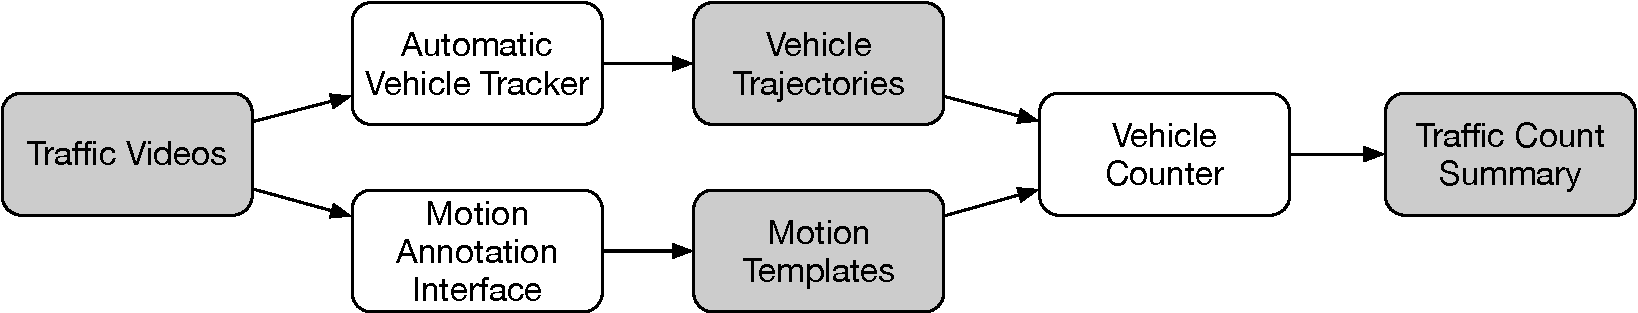
\includegraphics[width=\linewidth]{./img/system/kf-counter.pdf}
\caption{Vehicle counter workflow with human annotation.}
\label{fig:kf-counter}
\end{figure}
\begin{figure}
\centering
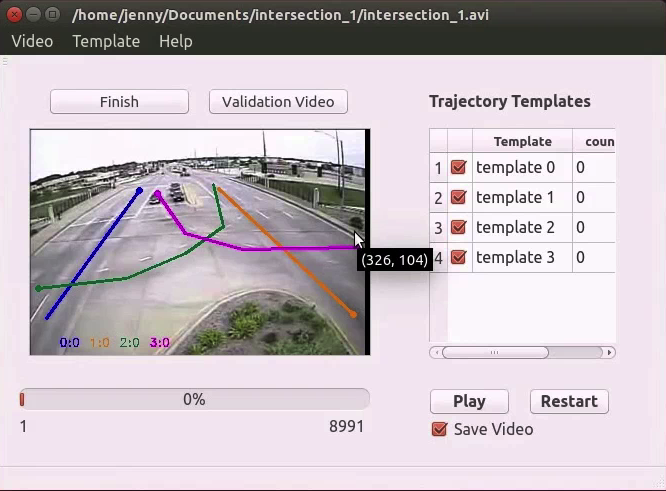
\includegraphics[width=\linewidth]{./img/system/line_seg.png}
\caption{Motion annotation interface.}
\label{fig:anno-gui}
\end{figure}

Suppose we have a set of $n$ motion templates $\mathbf{T} = \{\mathbf{T}_1, \mathbf{T}_2, \dots, \mathbf{T}_n\}$. 
Each template consists of segments $T_{m} = \{s_{1}, s_{2}, \dots, s_{m_l}\}$ and $s_{m_\cdot}$ is a line segment, $m_{l}$ is the number of the line segments of template $T_m$.
There is also a set of trajectories of $N$ vehicles $\Omega= \{\mathbf{O}_1^1, \mathbf{O}_1^2, \dots, \mathbf{O}_1^{t_1}, \mathbf{O}_2^1, \mathbf{O}_2^2, \dots, \mathbf{O}_2^{t_2}, \dots, \mathbf{O}_N^1, \mathbf{O}_N^2, \dots, \mathbf{O}_N^{t_N}\}$, where $t_i$ is the lifetime of object $i$.
Each object is matched to the template with the minimal maximal distance.
\begin{align}
T_i^* = \argmin_{T}{\avg_{t\in\{1, \dots, t_i\}}{D(O_i^t, T)}}.
\end{align}
$d(O_i^t, T)$ is defined as the minimal distance between the trajectory point and motion template $T$, measuring the distance and direction consistency at the same time:
$$d(O_i^t, T_m) = \min_{s\in\{T_m\}}{d(O_i^t, s)\cdot e^{-\alpha\cos(p(O_i^t, s))}}.$$
$d(O_i^t, s)$ is the perpendicular distance of a point to the line segment $s$, 
while $p(O_i^t, s)$ is the angle between $s$ and the moving direction of object $O_i$ at time $t$.
$\alpha$ is a constant, currently set as 1.

We develop the following template matching algorithm to ensure the trajectory is matched to the template that fit its motion most.
We start matching from the most confident trajectory point and continue matching until reaching the source and sink point of the trajectory.
Here the order of their closest segment was considered: all the trajectory points are not matched to the line segments of its previous trajectory point.
$s^{it}$ is defined as the closest segment of $O_i^t$, which is the $t$th point of object $i$'s trajectory. 
The distance $D(O_i^t, T)$ of object $O_i$ to template $T_m$ was computed as follows:
\begin{itemize}
\item Find the time $t^*$ such that $t_* = \argmin_{t\in\{1, \dots, t_i\}}{d(O_i^t, T_m)}$ and its closest segment $s^{it^*}$.
\item For the points before $O_i^{t_*}: O_i^{t}\in\{O_i^{1}, O_i^{2}, \dots, O_i^{t_-1}\}$, the closest segment falls in the first line segment of $T_m$ to its successor’s closest segment:
 $$D(O_i^t, T_m) = \min_{s\in\{s_1, s_2, \dots, s^{it-1}\}}{d(O_i^t, s)\cdot e^{-\alpha\cos(p(O_i^t, s))}}.$$
\item For the points after $O_i^{t_*}: O_i^{t}\in\{O_i^{t^*+1}, O_i^{t^*+2}, \dots, O_i^{t_i}\}$, the closest segment falls in its predecessor’s closest segment to the last line segment of $T_m$:
 $$D(O_i^t, T_m) = \min_{s\in\{s^{it^+1}, \dots, s_{m_l}\}}{d(O_i^t, s)\cdot e^{-\alpha\cos(p(O_i^t, s))}}.$$
\end{itemize}

By defining the distance function $D(\cdot)$ with both spatial distance and direction consistency and keeping the closest segment order, we eliminate close segments with inconsistent directions. 
Finally, the number of trajectories belonging to each template is the desired vehicle count.

\subsection{Vehicle counter with semantic knowledge}
\ref{fig:semantic-counter} shows the workflow of the improved counter with semantic knowledge. 
After offline learning in \S\ref{sec:scene-hdp}, the distribution of visual topics are learned; and each of them is a parameterized model.
In the tracking process \S\ref{sec:semantic-inf}, the fitting of each tracked vehicle with every model is examined by online inference.
In other words, the motion of the tracked vehicle is determined by the most fitted motion model. 
By increasing the vehicle count of each vehicle's motion upon leaving, counting can be done along with tracking. 

\begin{figure}
\centering
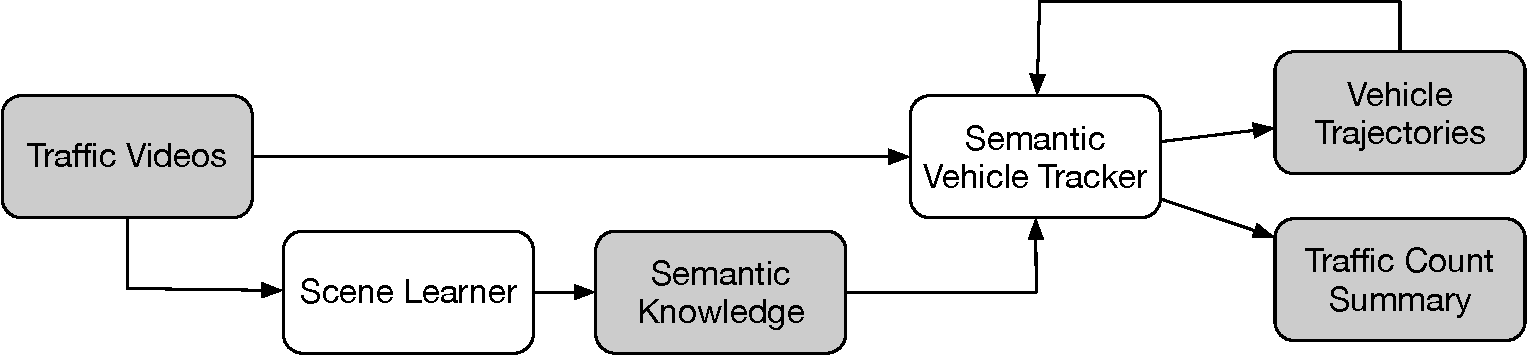
\includegraphics[width=\linewidth]{./img/system/semantic-counter.pdf}
\caption{End-to-end vehicle counter workflow with scene understanding.}
\label{fig:semantic-counter}
\end{figure}

\subsection{Web portal}
Based on the feedbacks from \gls{idot} about our previous GUI interface, we build a web portal of this system that integrates all the previous functions.
Currently, the system only supports manual template annotation as in \ref{fig:kf-counter}, the scene understanding module has not been integrated.
\ref{fig:sys-main} is the main interface of camera display: cameras are displayed on the map, with a list of their name on the left. 
Users may create or browse cameras by list or on the map, and upload videos for each camera. 
Similar to our previous GUI, once a new camera is created and the first video is uploaded, the user needs to draw the motion templates.
Then the tracker and counter are executed sequentially in the background. 
Users may return later to check the progress and download the results. We allow at most four videos processed at the same time. 
\ref{fig:sys-camera} and \ref{fig:sys-video} are the interface for camera and videos. 
Each camera may have multiple videos, all its videos, and their count summary is displayed on the left in the camera view. 
Clicking a video on the list leads to its individual video view. The video is played and detailed counts on each motion are displayed.
\begin{figure}
    \centering
    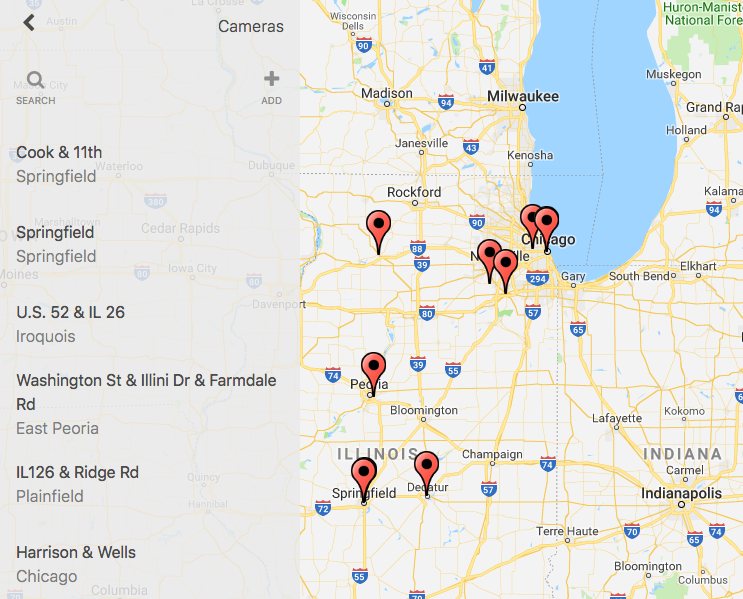
\includegraphics[width=\linewidth]{./img/system/main.png}
    \caption{Main interface of the web portal, cameras are displayed on the map.}
    \label{fig:sys-main}
\end{figure}
\begin{figure}
    \centering
    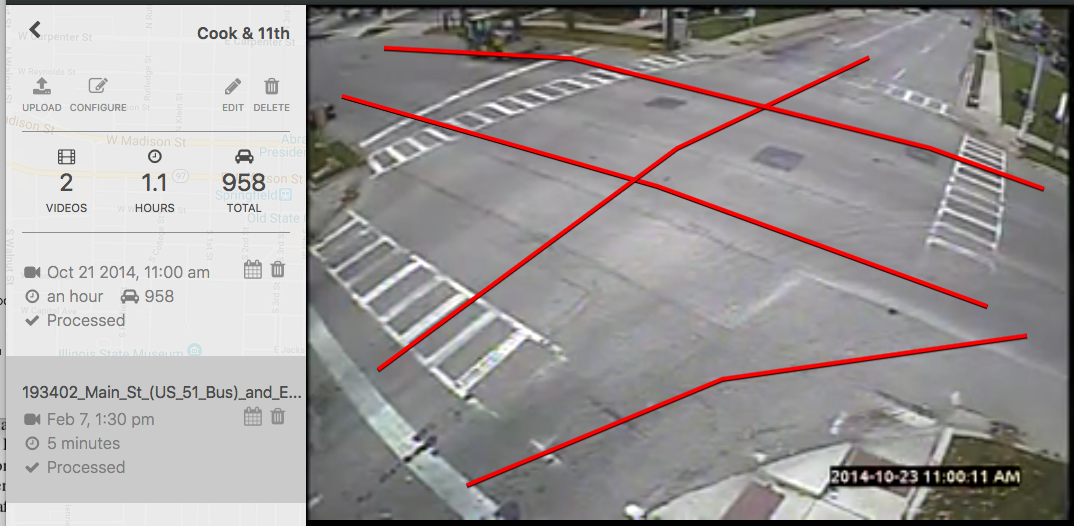
\includegraphics[width=\linewidth]{./img/system/camera.png}
    \caption{Camera view with video list and summary.}
    \label{fig:sys-camera}
\end{figure}
\begin{figure}
    \centering
    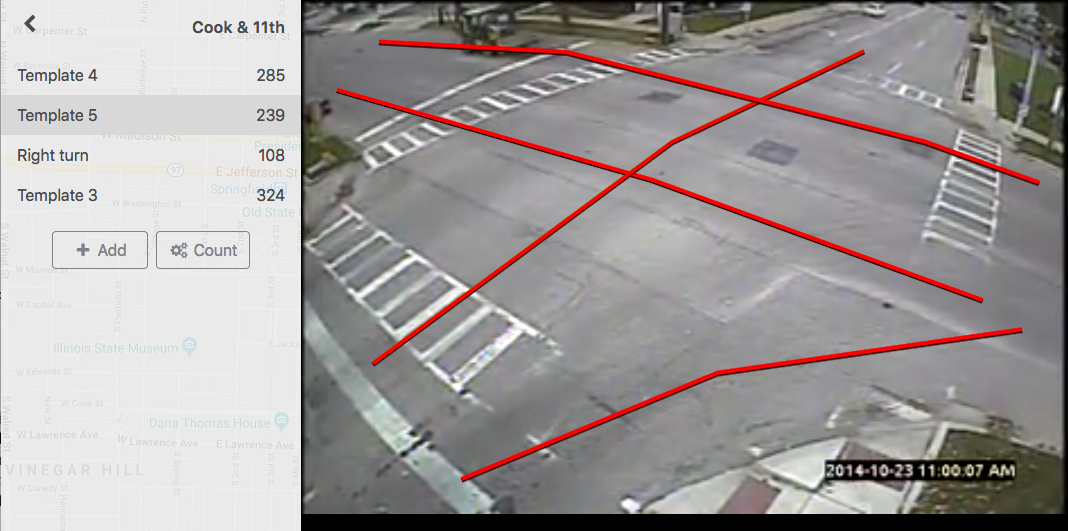
\includegraphics[width=\linewidth]{./img/system/video.png}
    \caption{Individual video view with counting information.}
    \label{fig:sys-video}
\end{figure}
